\section{Data Cleaning Survey}
Between April 2015 and Dec 2015, we conducted two sets of surveys and interviews with engineers, data analysts, and scientists who self-reported that they directly work with data in their organizations (N=29).

\subsection{Methods}\label{sec:survey}
The surveys consisted of a series of quantitative questions about tool/language preference and job description, and several open-ended questions about the participants' organization's data management challenges. The interviews followed the script of the surveys and audio was recorded.
It is important to note that we conducted two separate surveys to ensure that our survey questions were properly calibrated.
The first survey was conducted with a preliminary set of 53 questions in June 2015, and we collected 5 written responses and 4 in-person/phone interviews.
In November 2015 we conducted a revised second survey with 18 more focused questions, and collected 21 written responses. 
Most of the participants were contacted personally by the authors and were often acquaintances.
However, the authors took care to ensure that the participants were not informed of any of the quantitative hypotheses or conclusions of the study before taking the survey. 
Other participants were reached through forums frequented by data analysts\footnote{http://reddit.com/r/datascience}, and all participants had the option to take the survey anonymously.

It is important to note that this survey is not meant to be a statistically representative sample of industrial practice, and the number of participants is insufficient to draw statistically significant conclusions. Therefore, we present qualitative results around the insights learned from the participants, and contextualize these insights based on the participants' self-reported demographics.
The questions used in surveys one and two are available at \url{https://www.surveymonkey.com/r/data-cleaning} and \url{https://www.surveymonkey.com/r/YT8RP3R} respectively.

\subsubsection{Participant Demographics}
The survey asked a series of questions about the participants' job descriptions, expertise, and use of certain tools/interfaces.
We briefly summarize the results.

\vspace{0.5em}

\noindent\textbf{Job Descriptions: } We requested participants to provide a job description and details about their organizations. We categorized the participants by their reported organization size and their roles. The participants were mostly from larger organizations (defined as > 100 employees). We also found that they were mostly evenly split between infrastructure and data analytics. A surprisingly large number (7/30) reported that they performed both roles in their organizations. The results are summarized in Table \ref{tab:jobs}. 

\begin{table}[t]
\centering
\begin{tabular}{l|r}
%\hline
Size                               & Number \\
\hline
Small    & 7      \\
%\hline
Large & 17     \\
%\hline
N/A                                & 5\\  %\hline  
\end{tabular}
\quad
\begin{tabular}{l|r}
%\hline
Job Desc.                              & Number \\
\hline
Infrastructure    & 10      \\
%\hline
Analysis & 12     \\
%\hline
Both                                & 7\\  %\hline  
\end{tabular}

\caption{Categorized responses to the question ``Describe your company/organization and your role there.'' We defined a large organization as one with > 100 employees. To determine the job description, there was a clarifying question ``I develop infrastructure to process incoming and historical data at scale for use by other business units.". \label{tab:jobs}}
\end{table}

\vspace{0.5em}
\noindent\textbf{Data Products: } Machine Learning is an increasingly popular use-case for large datasets. We asked participants who self-reported as data analysts whether they work with Machine Learning. We found that 11/17 ``data analyst'' participants reported working with machine learning models.

\vspace{0.5em}
\noindent\textbf{Tools/Interfaces For Cleaning: } Next, we asked participants about the existing tools and interfaces they used for data cleaning. This set of questions was only asked in the second survey. Figure \ref{fig:interfaces} shows the results. We find that most of the participants responded that they used Python/Perl or MapReduce-like frameworks (clarified in the survey to be Spark/Hadoop etc.) to manipulate data before analysis. A minority of participants responded that they used graphical interfaces or rule-based interfaces to clean data.

\begin{figure}[t]
\centering
 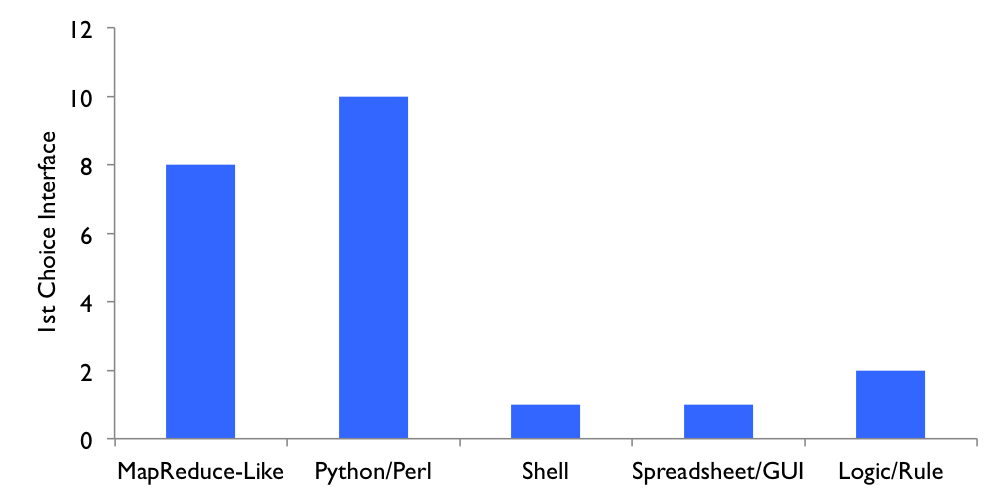
\includegraphics[width=\columnwidth]{datafigs/hilda-interface.png}
 \caption{Top ranked responses to: ``Which of the following tools/interfaces/languages do data scientists at your organization prefer for manipulating data, including extraction, schema transformations, and outlier removal, to make analysis easier or more reliable. Please Rank.''\label{fig:interfaces}}
\end{figure}


\subsection{Themes}\label{sec:themes}
We highlight several of the themes we discovered from the survey and the interviews: data cleaning methodology and the tension between infrastructure engineers and data analysts.

\subsubsection{Data Cleaning Methodology}
Among those participants who self-reported as data analysts, one major concern was data cleaning methodology.
Confirming the findings of Kandel et al., we afound that many participants reported data cleaning to be an interactive and iterative process, and as one participant noted,

\vspace{0.7em}
\emph{[It's an] iterative process, where I assess biggest problem, devise a fix, re-evaluate. It is dirty work.}

\vspace{0.5em}

We broadly interpreted iteration to mean that analysts alternate between cleaning data and analysis, and using the analysis to guide future cleaning cleaning results.
A natural concern raised by this approach is over-fitting: cleaning data until the output of a specific analysis is achieved.
We asked questions to explore how this iterative process may affect results, especially in the context of confirmation bias.

The next question that we asked was about evaluation methodology, namely, ``How do you determine whether the data is sufficiently clean to trust the analysis?'', and it was clear from the responses that many analysts had not thought about this problem:

\vspace{0.5em}
\emph{Other than common sense we do not have a procedure to do this.}

\vspace{0.7em}
\emph{We usually do not do rigorous validation of data cleaning. We typically clean our data until the desired analytics works without error. This is not desirable but practical since in most cases data error is probably overshadowed by errors/inaccuracies in the models themselves.}

\vspace{0.5em}

Iteration coupled with a lack of evaluation methodology is particularly worrisome.
In their defense, some analysts were aware of the potential of such problems, but did not have a solution.
For example, One analyst suggested comparing to other published results as a sanity check:

\vspace{0.5em}
\emph{We typically cross-reference data with other published materials to make sure it is in the right ballpark.}
\vspace{0.5em}

This is a solution may work in some cases, but many data analysis projects in industry are one-of-a-kind, and for most there likely does not exist a publicly available gold standard against which to validate results.
These results emphasize that the data cleaning community needs to have a better answer to this problem, especially in the backdrop of the reproducibility crisis in science~\cite{reproducibility}.

\subsubsection{Analysts vs. Infrastructure}
Another important theme that we discovered in the data was the divide between infrastructure engineers and analysts in how these groups address data quality problems. In particular, we see a difference in the way that these two groups of participants conceptualize dirty data, the solutions, and repair procedures.

One of the most significant tensions between the infrastructure engineers and analysts is about the definition of dirty data. While the infrastructure engineers are in charge of the data ingest pipelines, ETL, and other pre-processing steps, it is often the analysts who get to ``define'' what is dirty. One infrastructure engineer noted the frustration about being caught in the middle between the business units that generated the data and the analysts querying the data:

\vspace{0.5em}
\emph{There are often long back and forths with senior data scientists, devs, and the business units that provided the data on data quality. It is almost never a smooth process. The vast majority of problems are in turning semi-structured data into features. What placeholder value is sensible to use for a missing value, do we replace it with the mean or nearest neighbor; or is a variable ordinal or categorical? These are tough questions that often can only be answered by the business unit themselves. We try to get them to do some of this work but it inevitably falls on us esp. if it is a big unit.}

\vspace{0.5em}

The tension between the infrastructure engineers and the data analysts seems to stem from the semantics of data and who knows these semantics. Our responses also suggest that the definition of data error is highly analysis-dependent. In response to how she defines dirty data, one analyst responded,

\vspace{0.5em}
\emph{Domain expertise, I guess. I wish there were a more rigorous way to do this but we look at the models and guess if the data are correct.}

\vspace{0.5em}

This is in contrast to how infrastructure engineers want to handle data quality problems. 
Several infrastructure engineers noted that they saw dirty data as symptomatic of an error in the processing pipeline (i.e., a software bug or incorrect schema). Their goal was to rectify the bug or drop the corrupted data with a minimal impact on system SLOs:

\vspace{0.5em}
\emph{There are software bugs in the application such as edge cases that are not handled or changes to the services by programmers that have unintended consequences. Fixing data errors in a high-availability setting is challenge as it may require shutting off services.}

\vspace{0.5em}

Most of the infrastructure engineers surveyed used sampling or unit testing to detect obvious problems in the data processing pipeline, for example,

\vspace{0.5em}
\emph{We have checks for file consistency, if the end of files look like the write was interrupted early, whether the size of a file seems significantly bigger or smaller than usual, etc. we check data with some standard queries to make sure the files have the expected range of values, ie for every country, and every minute of the day there was data.}

\vspace{0.5em}

Such approaches require a clear definition of dirty data that is independent of the downstream analysis. Even worse, one consultant from a large database vendor noted that errors might be found well after some result is reported:

\vspace{0.5em}
\emph{Most of these errors are subtle enough that the analysis will go through e.g., with standard null value semantics of SQL, but give an incorrect answer. Usually is only caught weeks later after someone notices something like...well the Wilmington branch cannot have 1M sales in a week.}